This chapter discusses the potential implementation of the systems we discuss as a physical, chemical system. It is also possible to design as a sensor that connects to a traditional architecture, like \gls{cmos}, but we focus on a exclusively chemistry implementation here. We believe that the examples we discuss at the beginning of this work would benefit more as a full chemical system rather than a hybrid or sensor-system approach. We will first talk about various ways to map the system to a wet chemistry and how then fast the system would operate with state of the art.

\section{Chemical Representation}
In Chapter~\ref{chap:delay_line} and Chapter~\ref{chap:trail_simulations}, we used a set of reactions and species to represent our systems using the models of Michaelis\hyph Menten~\cite{Henri1903-jf}~\cite{Michaelis1913-zv}~\cite{Leskovac2003-ei} and mass-action kinetics~\cite{Horn1972-ob}~\cite{Erdi1989-ll}. Present work has mapped these set of rate reactions to different physical realizations. One such work is by Arkin and Ross, who implement a series of enzymatic gates that correspond to a truth table for a given logic function~\cite{Arkin1994-bs}. Arkin and Ross show that it is possible to implement both a logical AND and OR using a \gls{ggtca} model. Kompa and Levine use different chemical compounds that react at a faster rate to build similar types of logic gates to Arkin and Ross~\cite{Kompa2001-yk}.

Another applicable mapping for our work a \gls{dna} strand displacement model from Zhang and Seelig~\cite{Zhang2011-ey}. In this paper, Zhang and Seelig demonstrate the construction of a \gls{dna} walker that is capable of decision making with the use of only proteins. Similarly, Semenov \textit{et al.}~\cite{Semenov2014-bv} showed a more complex version of the walkers (that they called spiders) that have the ability to move along \gls{dna} and manipulate or read values. Qian \textit{et al.} builds linear threshold circuits that also operate in \gls{dna} strand displacement models to solve logic gates like AND, OR, NOT, and XOR through the use of \gls{ann}-like structures. All three of these works demonstrate that it is possible to create a mapping of chemical reactions to physical, chemical systems. Using similar principles from these works, we could take our equations from Chapter~\ref{chap:trail_simulations} to a set of \gls{dna} strand displacement models that could achieve our desired result.

Stojanovic and Stefanovic have also shown how deoxyribozyme catalysis can be used to solve games like tic-tac-toe using 23 logic gates built at a molecular scale~\cite{Stojanovic2003-eg}~\cite{Stojanovic2000-qx}. Their system was capable, in a wet chemistry, of playing successful games of tic-tac-toe with human players using fluorescence as a detection method. Liu \textit{et al.} has also used dexoyribozyme catalysis to implement antibody and nucleic acid detectors~\cite{Liu2009-jz}. This technology is likely the best candidate of mapping our system to a wet chemical implementation. As a small example, we can show how something like the delay line would look mapping with similar technology to this.

Figure~\ref{fig:deoxy1} shows an example of a length two \gls{mdl} with the signals being the deoxyribozymes $X1_{signal}$ and $X2_{signal}$, which cleave the substrate $X$ at the embedded ribonucleotide. This produces $X1$ ready for the next system to consume. Subsequently, $X1C$ embedded with another ribonucleotide is able to get cleaved by deoxyribozyme $X2_{signal}$ to form the next input to the system, $X2$. This system is at a similar scale to that discussed in the work by Stojanovic \textit{et al.} Let us now take a look at implementation of a full trail solving system.

\begin{figure}[ht]
	\centering
	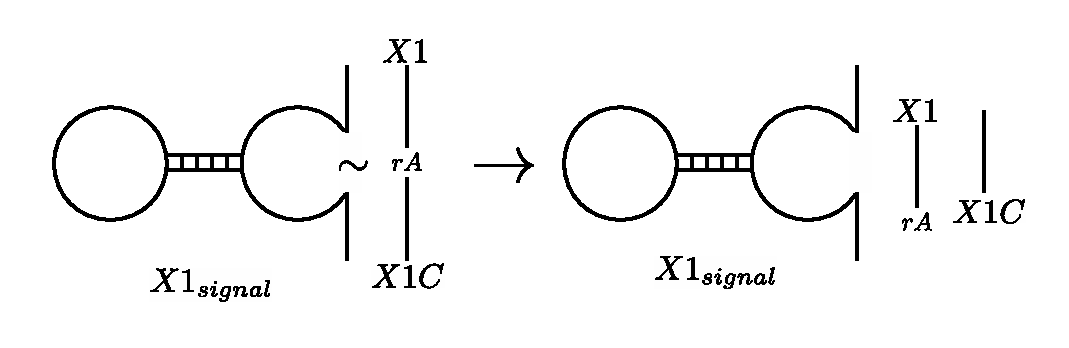
\includegraphics[width=12cm]{cleavage}
	\caption[Example of Deoxyribozyme Implementation]{Deoxyribozyme cascading example. Deoxyribozyme $X1_{signal}$ cleaves $X$ at embedded ribonucleotide ($rA$) to form $X1$ and $X1C$. A similar process occurs on $X1C$ to produce $X2$ and $X2C$.}
	\label{fig:deoxy1}
\end{figure}

We have discussed works operating typically on only a small region of \gls{dna} or representing only a few chemical reactions. The size of the system necessary to construct our full ant solver is much larger than these. For example, take the \gls{mdl} connected to the perceptrons in the previous chapter to form the \gls{ann} for our ant trail system. Each four- and five-input \gls{aasp} is composed of 33 and 38 reactions and 37 and 42 unique species, respectively. Recall from Chapter~\ref{chap:delay_line}, a four-input delay line requires eight reactions and 13 species. So, for an entire trail system with a hidden layer, this results in $8+33+3 \cdot 38=155$ reactions and $13+37+3 \cdot 42=176$ species for our system. This number of reactions and species is greater in complexity than other systems we have found presently implemented in a chemical system.

As an example, the four-neuron Hopfield associative memory from Qian \textit{et al.} contained around 160 reactions with 72 initial \gls{dna} species~\cite{Qian2011-nw}. While this system contained more reactions, the number of species co-existing in this system is less than half the number predicted for full computation of our trail system. One issue that Qian \textit{et al.} discuss in their work is that scaling up the system can amplify leak reactions that occurred and degrade performance of the overall system. Adding the increased number of species we require could have this type of issue. Another observation by Stojanovic and Stefanovic in their work was erroneous output by gates that should not be signalling. The authors mention that this behavior may lead to errors cascading in larger networks that may lead to undesired behavior~\cite{Stojanovic2003-eg}.

Taking a system, such as this today into a wet chemistry is not impossible, but perhaps difficult based on the current state of the art for the field. It seems that there is not a system of this scale presently implemented as a wet chemistry and other work by Qian \textit{et al.} mentions potential issues as their systems continued to grow in size. One area of improvement is perhaps looking at a way to reduce the complexity of the network in a \gls{crn}. With more work on complex network implementation in a \gls{crn}, in theory, it should be possible to map the trail system reactions with the methods used by Zhang and Seelig, Semenov \textit{et al.}, Stojanovic and Stefanovic, or Liu \textit{et al.} to a physical chemistry. Components of the system, like the delay line by itself, require a smaller number of reactions and may be more feasible for present implementation. If implemented in a wet chemistry, let us now discuss if we can predict the speed at which this system would operate based off current work.

\section{Processing Speed}
As discussed in the previous section, the applicable mapping of our work is likely the deoxyribozyme catalysis~\cite{Stojanovic2003-eg}~\cite{Stojanovic2000-qx}~\cite{Liu2009-jz}. Stojanovic and Stefanovic specifically find that 15 minutes is a reasonable time to cleave and accurately observe the results from the reactions in their tic-tac-toe system. The authors did observe that changing the size of the gates in the chemistry or the concentration of inputs did have an impact on the reaction time, but did not elaborate beyond that. Zhang and Seelig~\cite{Zhang2011-ey} also observe times in the scale of several minutes to compute similar systems in a \gls{dna} strand displacement model.

The advantage of the chemistry is the chemical reactions (for example, each calculation of output layer peceptron in our \gls{ann} controlling the ant) can occur in parallel. This of course assumes separation using the compartmental chemistry by Blount \textit{et al.}~\cite{Blount_undated-ro}. As an example, if we take the 15 minute time found by Stojanovic and Stefanovic per reaction, we can predict the cycle time for a single calculation in our trail system.

Let us start with the network in Figure~\ref{fig:chem_comp_dl4} and predict the time to complete a movement for the trail system. With a length four \gls{mdl}, that requires waiting on four steps to occur for shift and store the input value to each block of the delay line. Then, there is a required period of calculation at the hidden neuron followed by one in the output layer. The output layer perceptrons are all able to calculate their results in parallel unlike the delay line, which depends on previous inputs. 

So, in total, that gives six stages of calculation. With the 15 minutes found by Stojanovic and Stefanovic, that means approximately 90 minutes for a single calculation step for the full \gls{ann}. Running a full system with 200 steps of the John Muir trail would take approximately 12.5 days with this current technology. It is important to note as well that the time we are discussing here is the estimated time to reach a steady state. In a wet chemistry, all of the reactions are occurring in parallel, so a separation between the nodes represented in our \gls{ann} diagram is critical. 

Catalysts or other signaling methods are required to prevent the later nodes from consuming the species too early. For example in the delay line, we use our $Xn_{signal}$ species to perform this separation. Also, unlike in an electrical system, the inputs are consumed, meaning, that as we perform the calculation, we are actually decreasing the value of the input as the calculation occurs. 

Even though the value is over 12 days for this example, other architectures in chemistry may provide a faster run time. Kompa and Levine~\cite{Kompa2001-yk} discuss the use of different chemicals like aberchromes (I), fulgides, and merocyanines (II) that show dynamics faster than discussed from Stojanovic and Stefanovic. The authors even predict that with continued development of their work, it may be possible to see chemical reactions with photophysicochemical processes operating on a picosecond range.